%%% -*-LaTeX-*-
\documentclass[../Dissertation]{subfiles}

\doublespacing
\graphicspath{{Organization/media/}{media/}} % Graphics path for images

\begin{document}

\chapter[\uppercase{Thesis/Dissertation
Organization}]{\uppercase{Thesis/Dissertation \protect\\Organization}}

    To setup your Thesis/Dissertation, take advantage of the \hologo{LaTeX}
    package \href{https://ctan.org/pkg/subfiles}{\texttt{subfiles}} which
    allows you to break apart your document into various sections and compile
    them individually for editing purposes:
    
    \codeFromFile{LaTeX}
        {./Organization/fileStructure/Dissertation_Organization.tex} % 
        {\ldots \hologo{LaTeX} script used to setup the document.}
        {main}
        {\footnotesize}
        {latexcodebg}
        {default}

\section{Student Info Setup}
    \cref{code:StudentInfo} is used to specify student-specific information.  
    
    \codeFromFile{LaTeX}
        {\subfix{../StudentInfo.tex}}
        {\ldots \hologo{LaTeX} script used for Student-Specific Info.}
        {StudentInfo}
        {\footnotesize}
        {latexcodebg}
        {default}

\section{Individual \cref{chp:1} Setup}

    \codeFromFile{LaTeX}
        {\subfix{../Chapter1/Chapter1.tex}}
        {\ldots \hologo{LaTeX} script used for chapter 1.}
        {Chapter1}
        {\footnotesize}
        {latexcodebg}
        {default}

\section{Individual \cref{chp:2} Setup}

    \codeFromFile{LaTeX}
        {\subfix{../Chapter2/Chapter2.tex}}
        {\ldots \hologo{LaTeX} script used to import a chapter.}
        {Chapter2}
        {\footnotesize}
        {latexcodebg}
        {default}

\section{Individual \cref{chp:3} Setup}

    \codeFromFile{LaTeX}
        {\subfix{../Chapter3/Chapter3.tex}}
        {\ldots \hologo{LaTeX} script used to import a chapter.}
        {Chapter3}
        {\footnotesize}
        {latexcodebg}
        {default}

\section{Individual \cref{chp:4} Setup}

    \codeFromFile{LaTeX}
        {\subfix{../Chapter4/Chapter4.tex}}
        {\ldots \hologo{LaTeX} script used to import a chapter.}
        {Chapter4}
        {\footnotesize}
        {latexcodebg}
        {default}

\section{Individual \cref{chp:5} Setup}

    \codeFromFile{LaTeX}
        {\subfix{../Chapter5/Chapter5.tex}}
        {\ldots \hologo{LaTeX} script used to import a chapter.}
        {Chapter5}
        {\footnotesize}
        {latexcodebg}
        {default}

\section{Individual \cref{AppendixA} Setup}

    \codeFromFile{LaTeX}
        {\subfix{../AppendixA/AppendixA.tex}}
        {\ldots \hologo{LaTeX} script used to import an appendix.}
        {AppendixA}
        {\footnotesize}
        {latexcodebg}
        {default}

\section{Individual \cref{AppendixB} Setup}

    \codeFromFile{LaTeX}
        {\subfix{../AppendixB/AppendixB.tex}}
        {\ldots \hologo{LaTeX} script used to import an appendix.}
        {AppendixB}
        {\footnotesize}
        {latexcodebg}
        {default}

\section{Individual \cref{AppendixC} Setup}

    \codeFromFile{LaTeX}
        {\subfix{../AppendixC/AppendixC.tex}}
        {\ldots \hologo{LaTeX} script used to import an appendix.}
        {AppendixC}
        {\footnotesize}
        {latexcodebg}
        {default}

\section{How To Use This Thesis/Dissertation \hologo{LaTeX} Template?}
    In order to take advantage of the whole functionality of \hologo{LaTeX} to
    compile your Thesis/Dissertation, it is recommended to use a Linux system.
    This can be done on Microsoft Windows using the Linux subsystem
    \href{https://ubuntu.com/}{\texttt{Ubuntu}}.  The alternative is to use
    \href{https://www.overleaf.com/}{\texttt{Overleaf}} which takes care of all
    of the package installation requirements.  

\subsection{Overleaf Template}
    To get started using the Overleaf template (\cref{fig:Overleaf}), click the
    following link:
    \href{https://www.overleaf.com/latex/templates/university-of-utah-thesis-slash-dissertation-template/cvsmnmqjwtck}{University
    of Utah Thesis/Dissertation Template}.  You can begin writing as soon as
    you add the project to your ``cloud''.  Be sure to check that the
    ``Recompile'' option is set to ``off'' or else it will recompile each time
    you change \texttt{.tex} files.  When you want to compile hit the button or
    press ``\texttt{Ctrl + S}'' (\cref{fig:Overleaf_autocompile}).  The benefit
    of using overleaf is that you do not have get \hologo{LaTeX} installed on
    your local machine and you can preview the finished project on the same
    screen.  Just be careful when your project has a lot of figures and
    references that it will take time to compile when you press ``\texttt{Ctrl
    + S}'' to compile.  
    
    \begin{figure}[H]
        \centering
        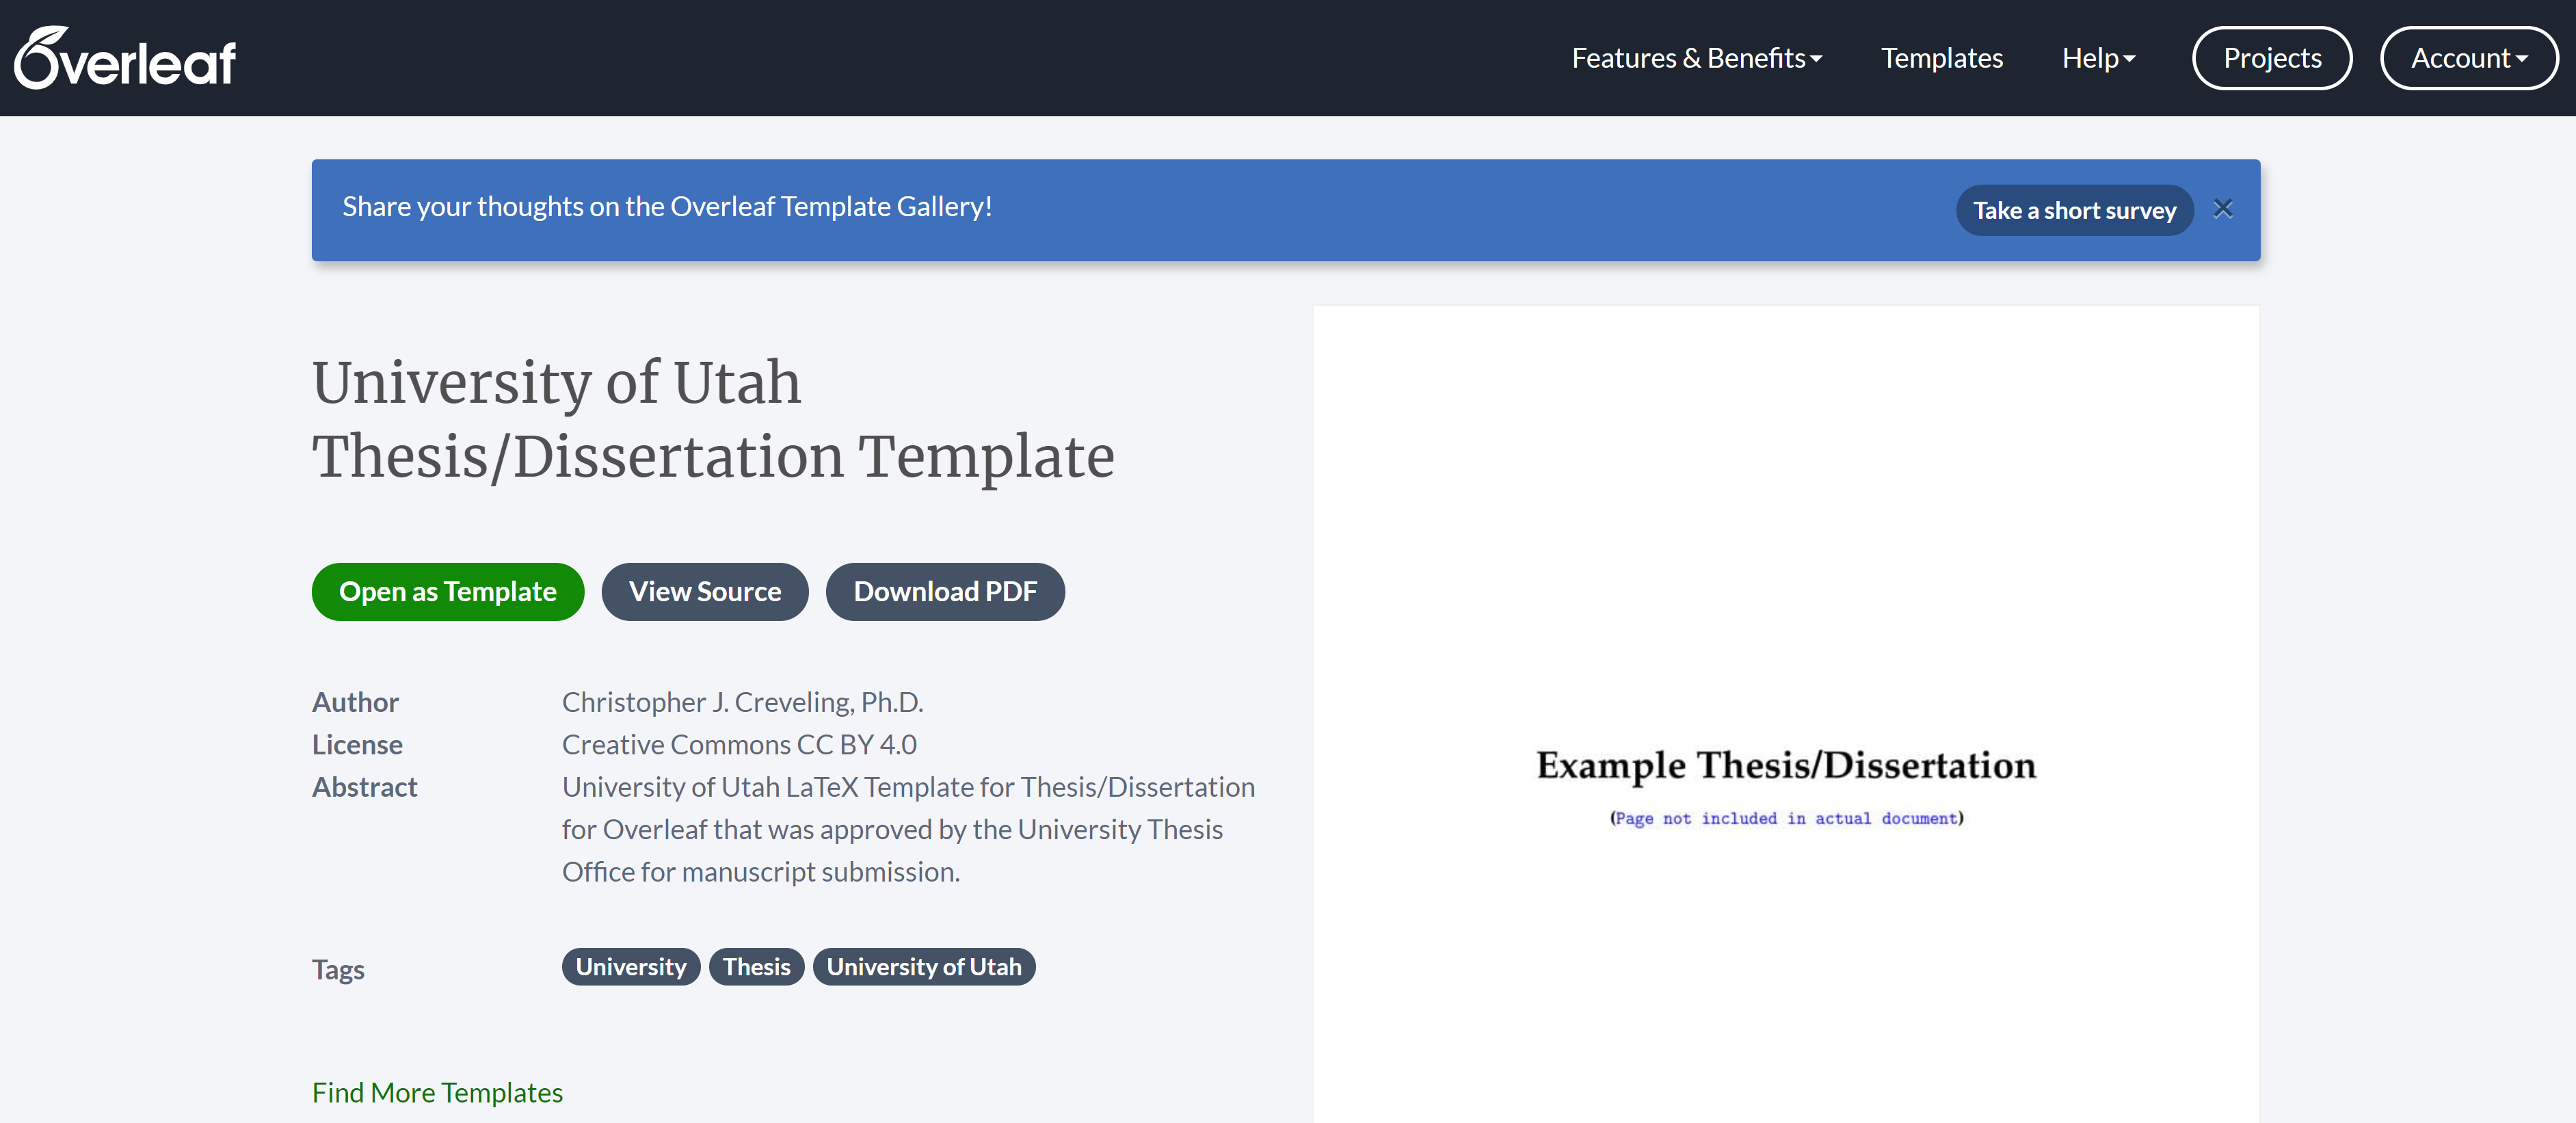
\includegraphics[width=0.8\textwidth]
        {./Overleaf}
        \caption{Overleaf project template.}
        \label{fig:Overleaf}
    \end{figure}
    
    \begin{figure}[H]
        \centering
        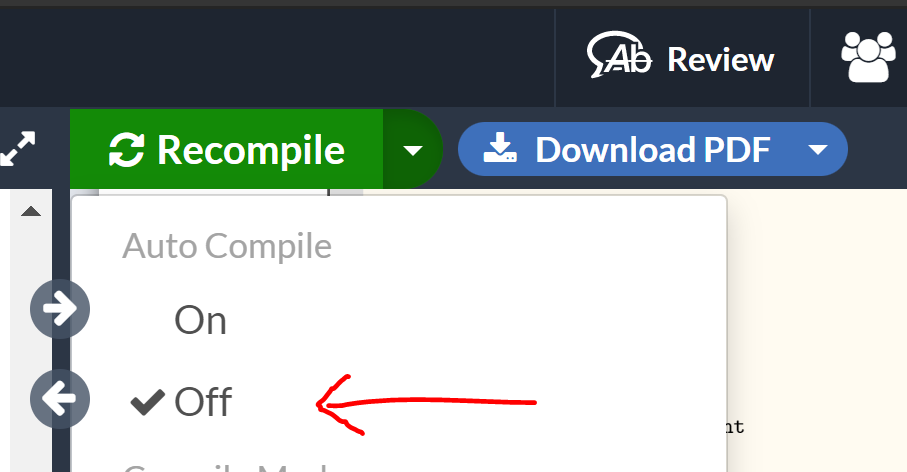
\includegraphics[width=0.5\textwidth]
        {./Overleaf_autocompile}
        \caption{Overleaf autocompile option.}
        \label{fig:Overleaf_autocompile}
    \end{figure}
    
\subsection{Steps to Get Writing using Linux}
    The primary advantage using this method to write your thesis/dissertation
    is that you can write when you are offline.  Another benefit of using this
    method is the files are on your local machine, you can open files as much
    as you'd like and you only compile/update when you specify. \\
    
    Below are the steps you will need to take to get your thesis/dissertation
    working on your local machine:
    \begin{enumerate}
        \item Enable the Linux subsystem for Windows (\cref{fig:LinuxSubsystem})
            \begin{figure}[H]
                \centering
                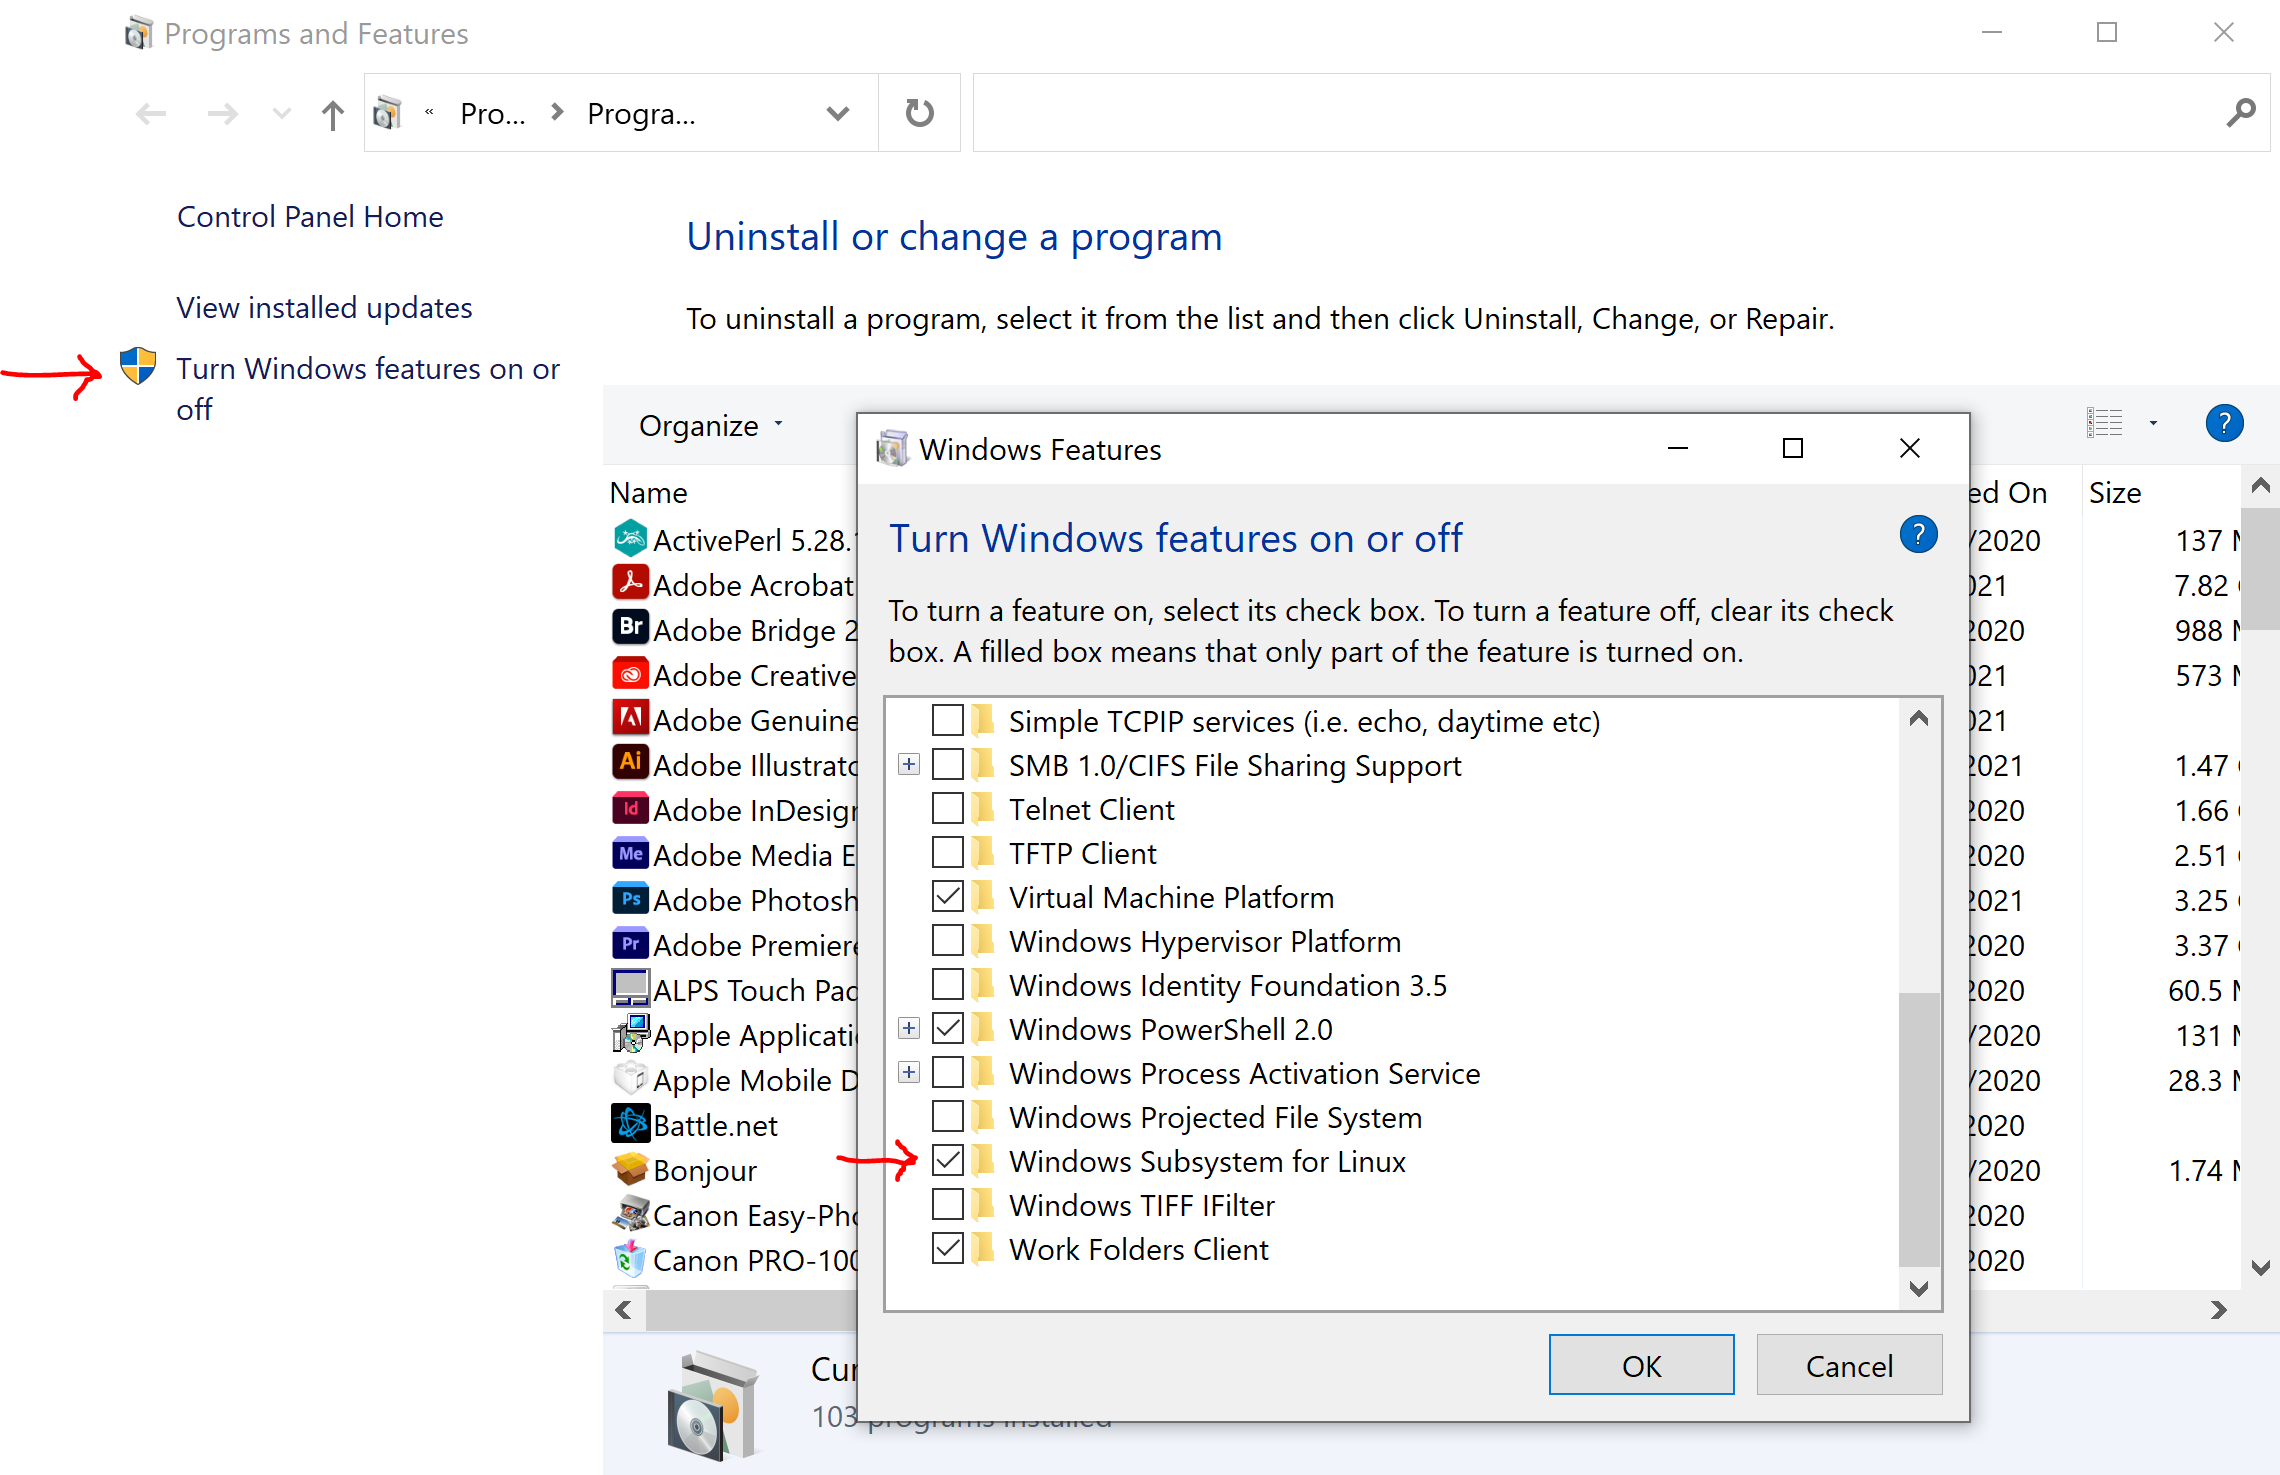
\includegraphics[width=1.0\textwidth]
                {./LinuxSubsystem}
                \caption{Enable Windows Subsystem for Linux}
                \label{fig:LinuxSubsystem}
            \end{figure}
        \item Download the Ubuntu application from the Microsoft App store
            (\cref{fig:UbuntuApp})
            \begin{figure}[H]
                \centering
                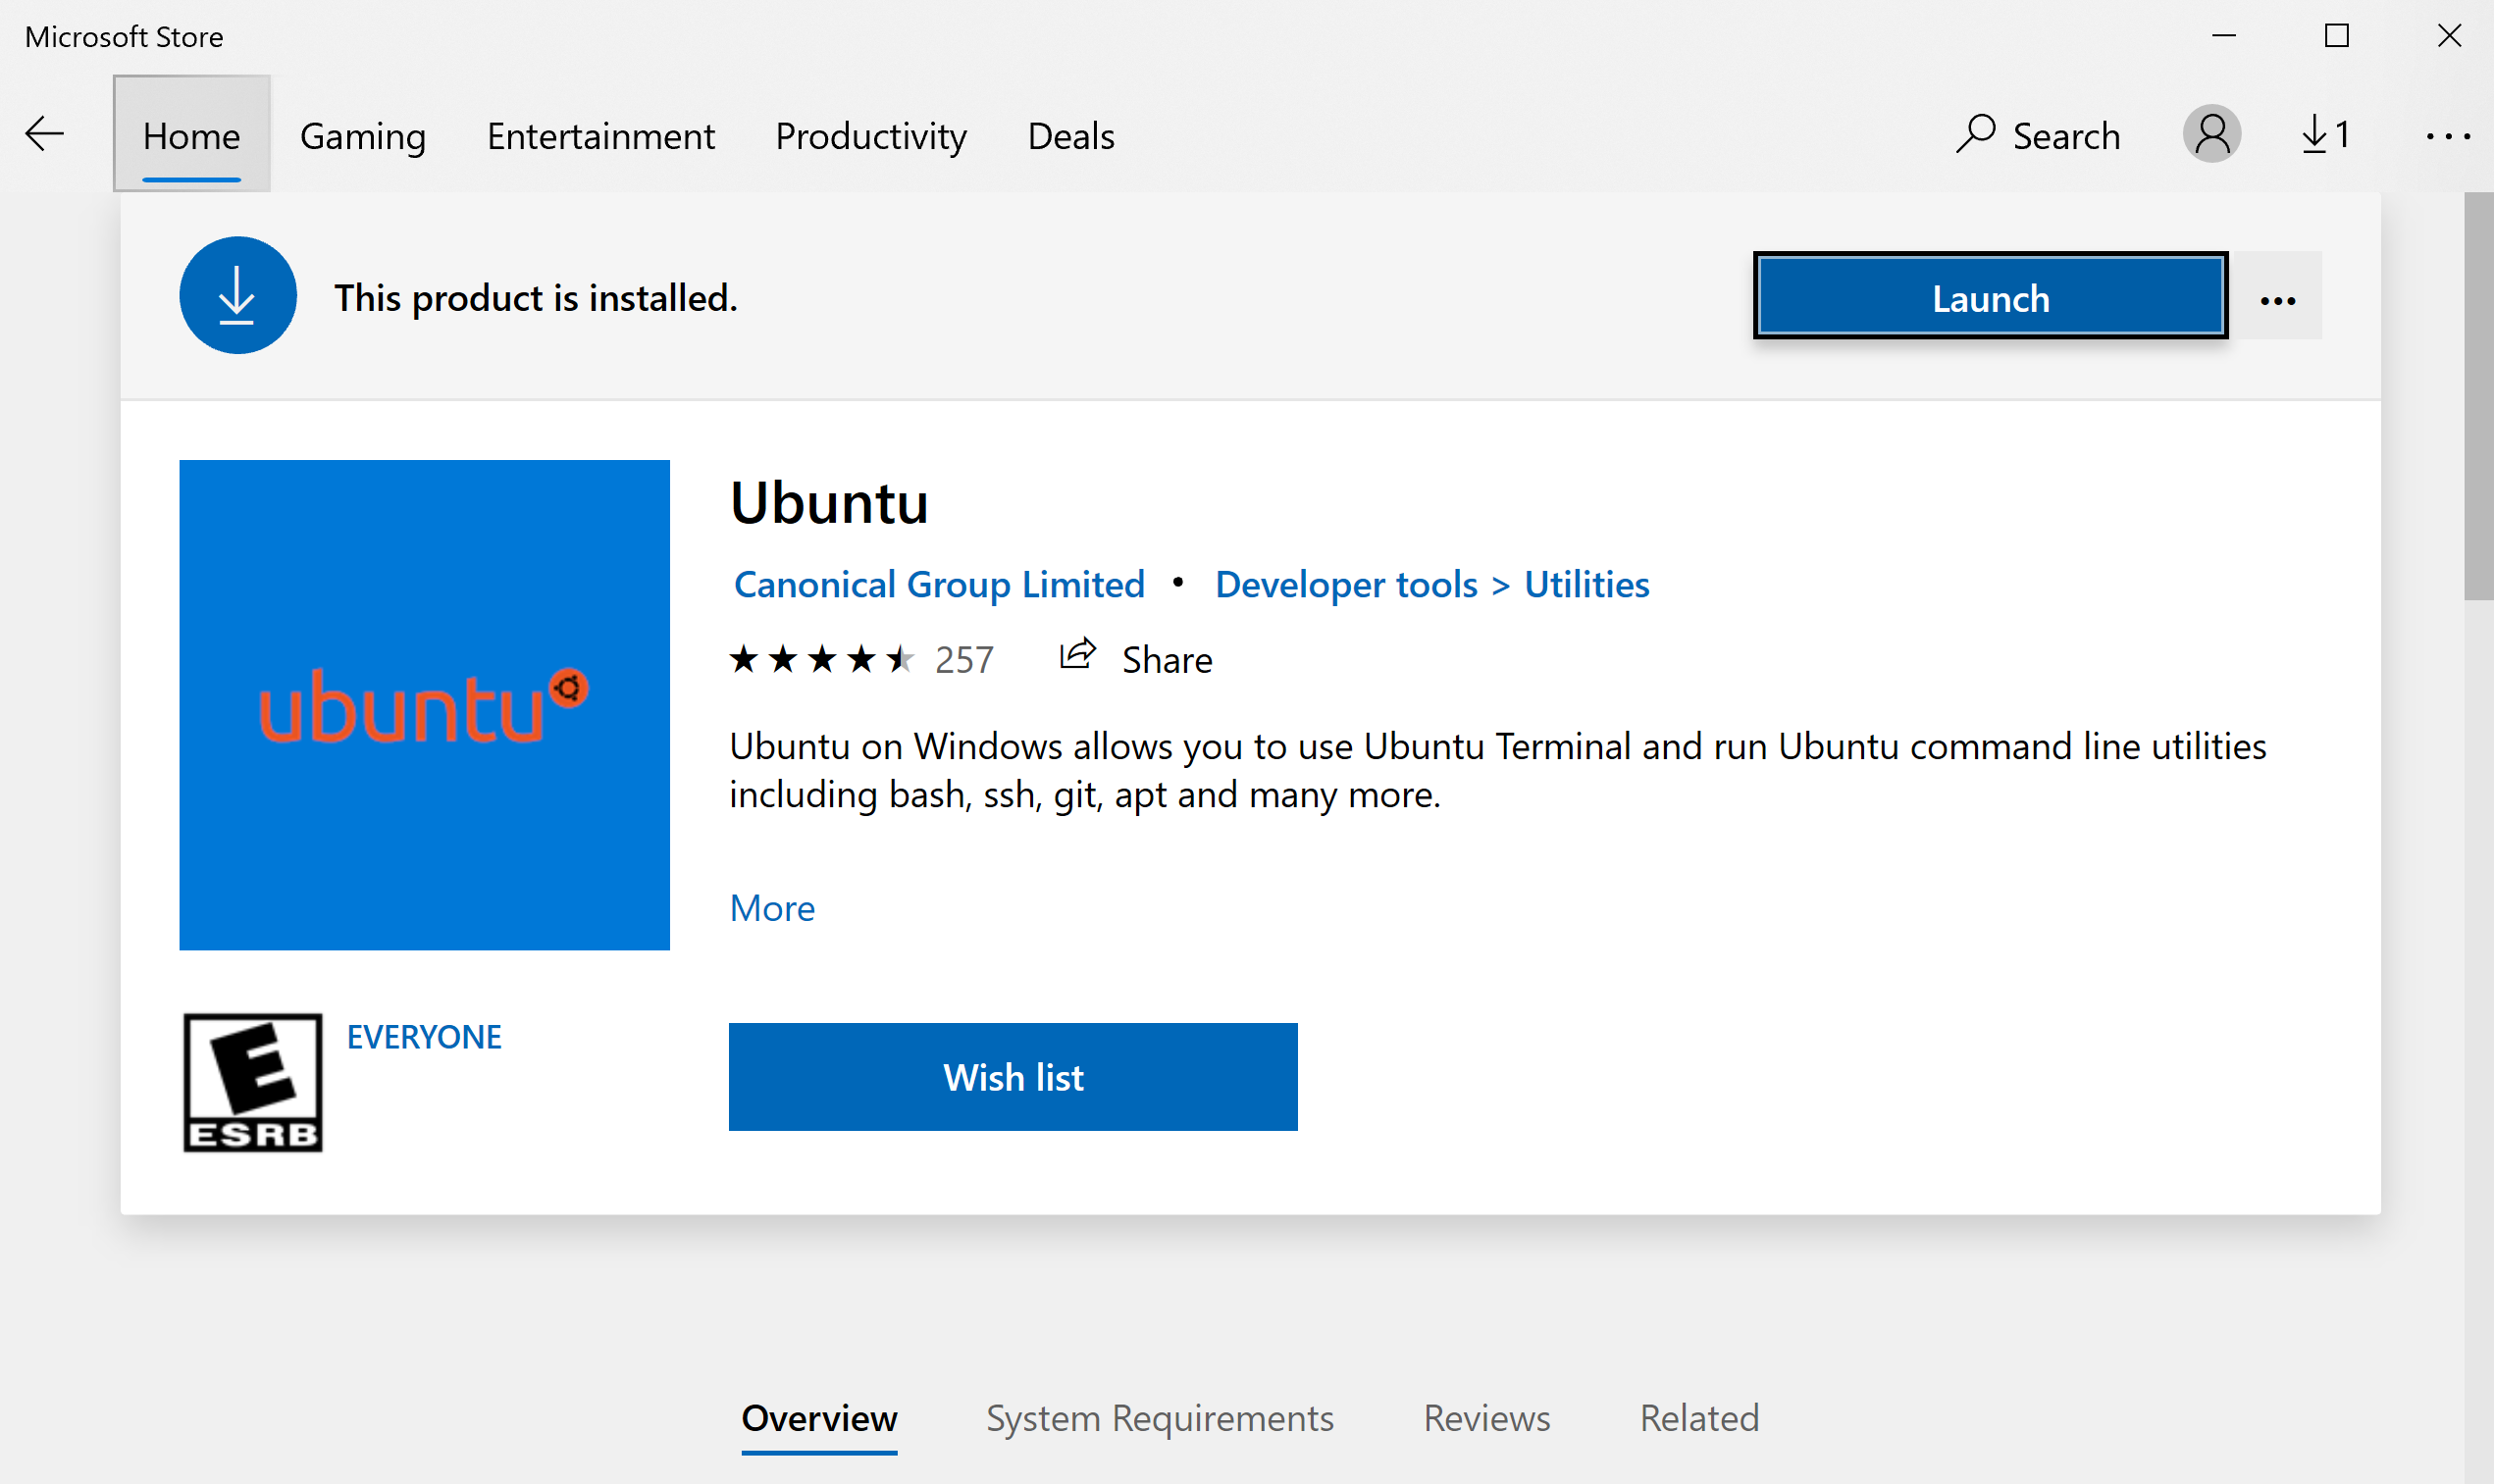
\includegraphics[width=1.0\textwidth]
                {./UbuntuApp}
                \caption{Download Ubuntu}
                \label{fig:UbuntuApp}
            \end{figure}
        \item Create a \href{https://gitlab.com/}{\texttt{GitLab}} account to
            pull files.  (You will learn how to do version control once you get
            your Thesis/Dissertation setup).  There is a fabulous link to learn
            the basics of \mintinline{Bash}{Git}:
            \href{https://docs.gitlab.com/ee/gitlab-basics/start-using-git.html}
            {https://docs.gitlab.com/ee/gitlab-basics/start-using-git.html}
        \item Initialize \texttt{Ubuntu} on your local machine and estabilish
            the connection to your own repository.
            {\singlespacing
            \begin{minted}
                [autogobble,bgcolor=latexcodebg] % 
                {Bash}
git config --global user.name "your_username"
git config --global user.email "your_email_address@example.com"
            \end{minted}
            }
        \item Clone the Thesis/Dissertation template to your local machine from
            the following link:
            \href{https://gitlab.com/SkiEngineer/uofuthesistemplate.git}{https://gitlab.com/SkiEngineer/uofuthesistemplate.git}.
            (\cref{fig:GitLabMain,fig:GitLabClone}).
            % \newline
            {\singlespacing
            \begin{minted}
                [autogobble,bgcolor=latexcodebg] % 
                {Bash}
git clone https://gitlab.com/SkiEngineer/uofuthesistemplate.git
            \end{minted}
            }
            \begin{figure}[H]
                \centering
                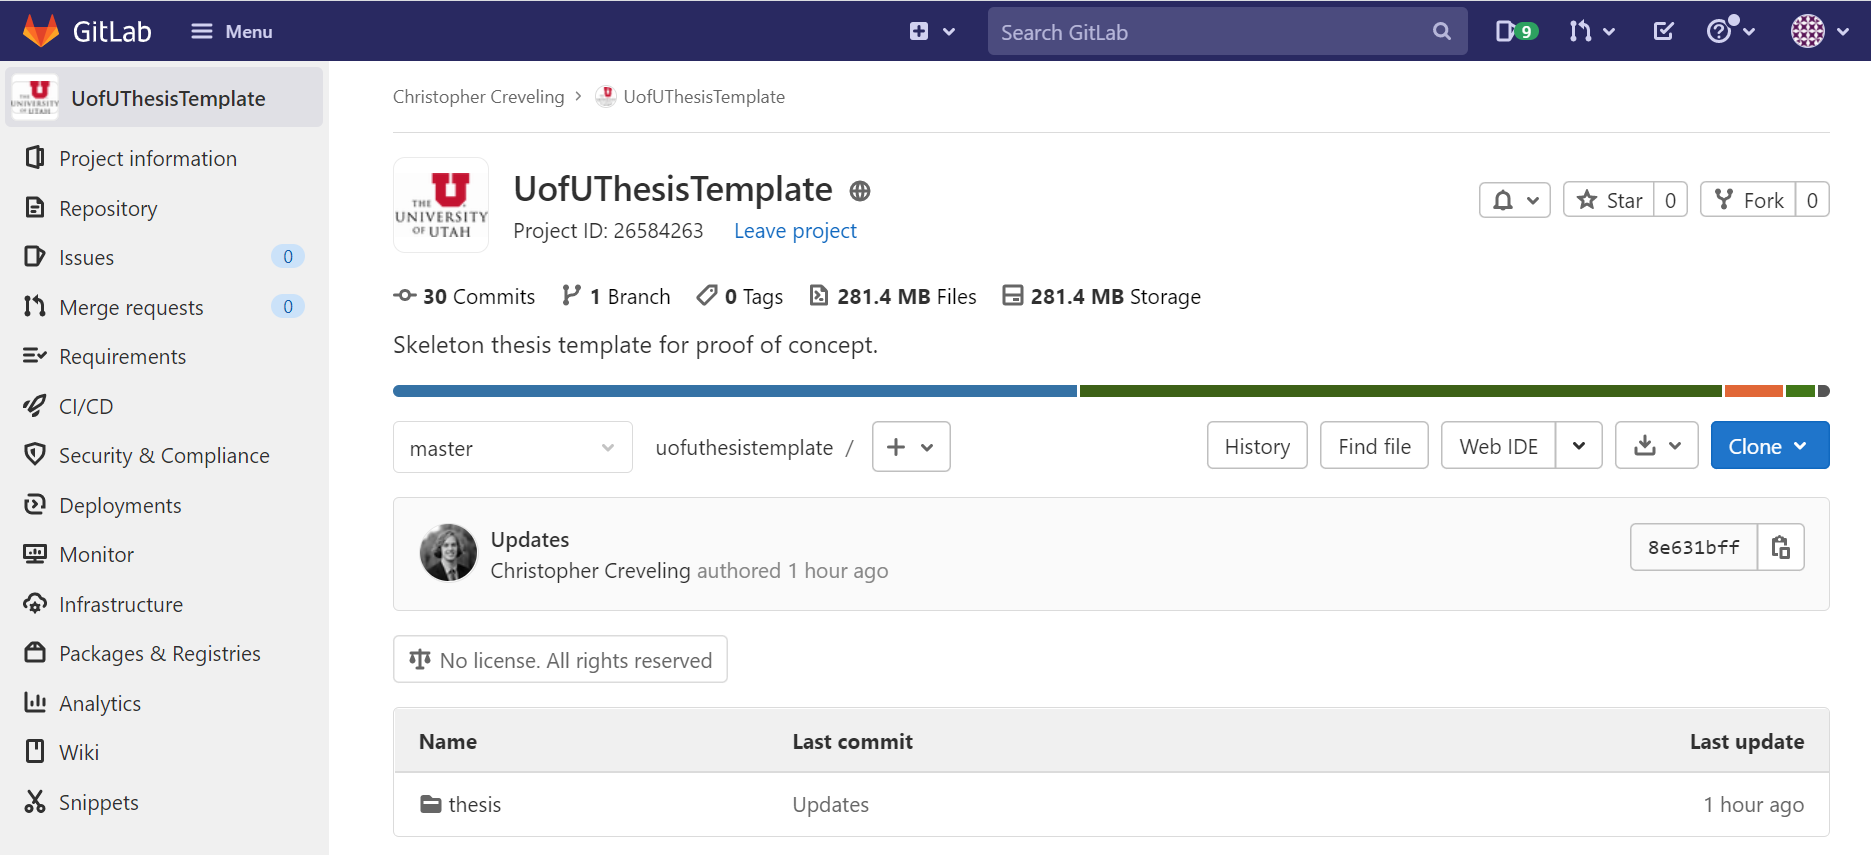
\includegraphics[width=1.0\textwidth]
                {./GitLabMain}
                \caption{GitLab main screen.}
                \label{fig:GitLabMain}
            \end{figure}
            \begin{figure}[H]
                \centering
                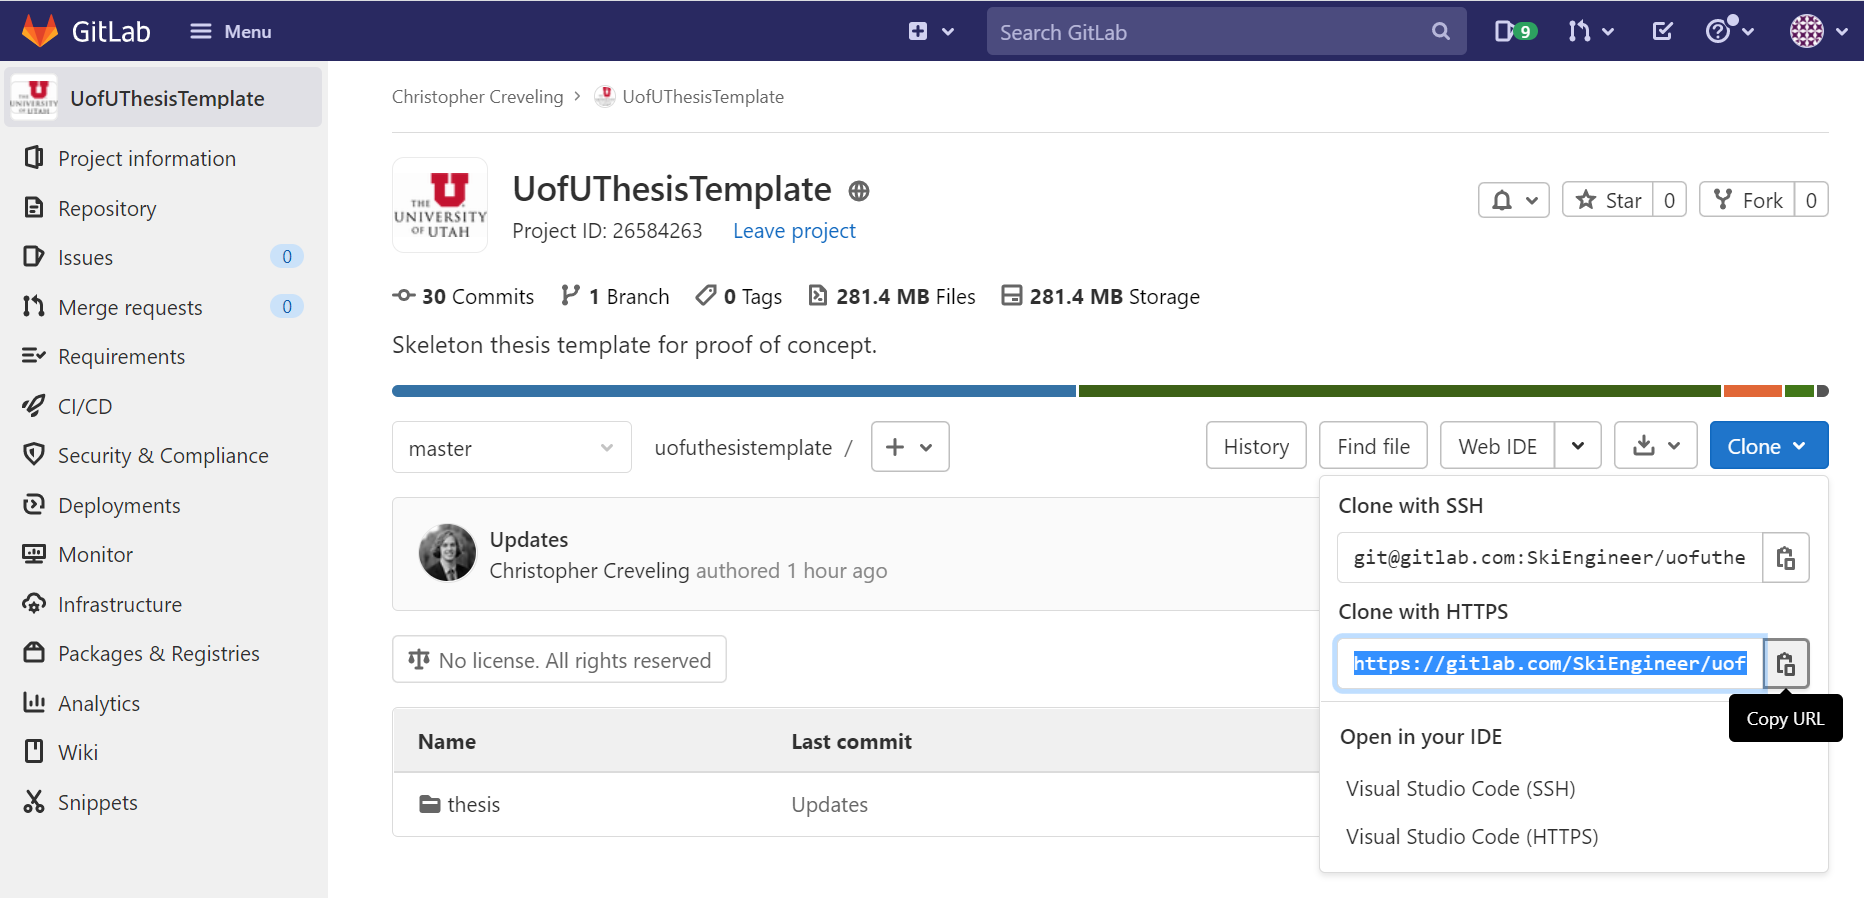
\includegraphics[width=1.0\textwidth]
                {./GitLabClone}
                \caption{Clone repository.}
                \label{fig:GitLabClone}
            \end{figure}
        \item In \texttt{GitLab}, create a new project titled:
            ``new\_awesome\_project'' (\emph{This will be the name of your
            Thesis/Dissertation}).  This is where you are going to put the
            Thesis/Dissertation template and make changes.  Create a new local
            directory titled:  ``new\_awesome\_project''.  Navigate inside the
            newly created folder and clone this ``new'' repository to your
            local machine.  See \cref{fig:GitLabClone} for details.  
            {\singlespacing
            \begin{minted}
                [autogobble,bgcolor=latexcodebg] % 
                {Bash}
git clone https://gitlab.com/SkiEngineer/new_awesome_project.git
            \end{minted}
            }
        \item Navigate to the ``\texttt{uofuthesistemplate}'' template folder
            directory and copy the files to your own Thesis/Dissertation folder
            on your local machine in the subsystem directory.  
            {\singlespacing
            \begin{minted}
                [autogobble,bgcolor=latexcodebg] % 
                {Bash}
cd ..
cd uofuthesistemplate
cp -r thesis ../new_awesome_project
            \end{minted}
            }
            (\cref{fig:gitLabProject}).
            \begin{figure}[H]
                \centering
                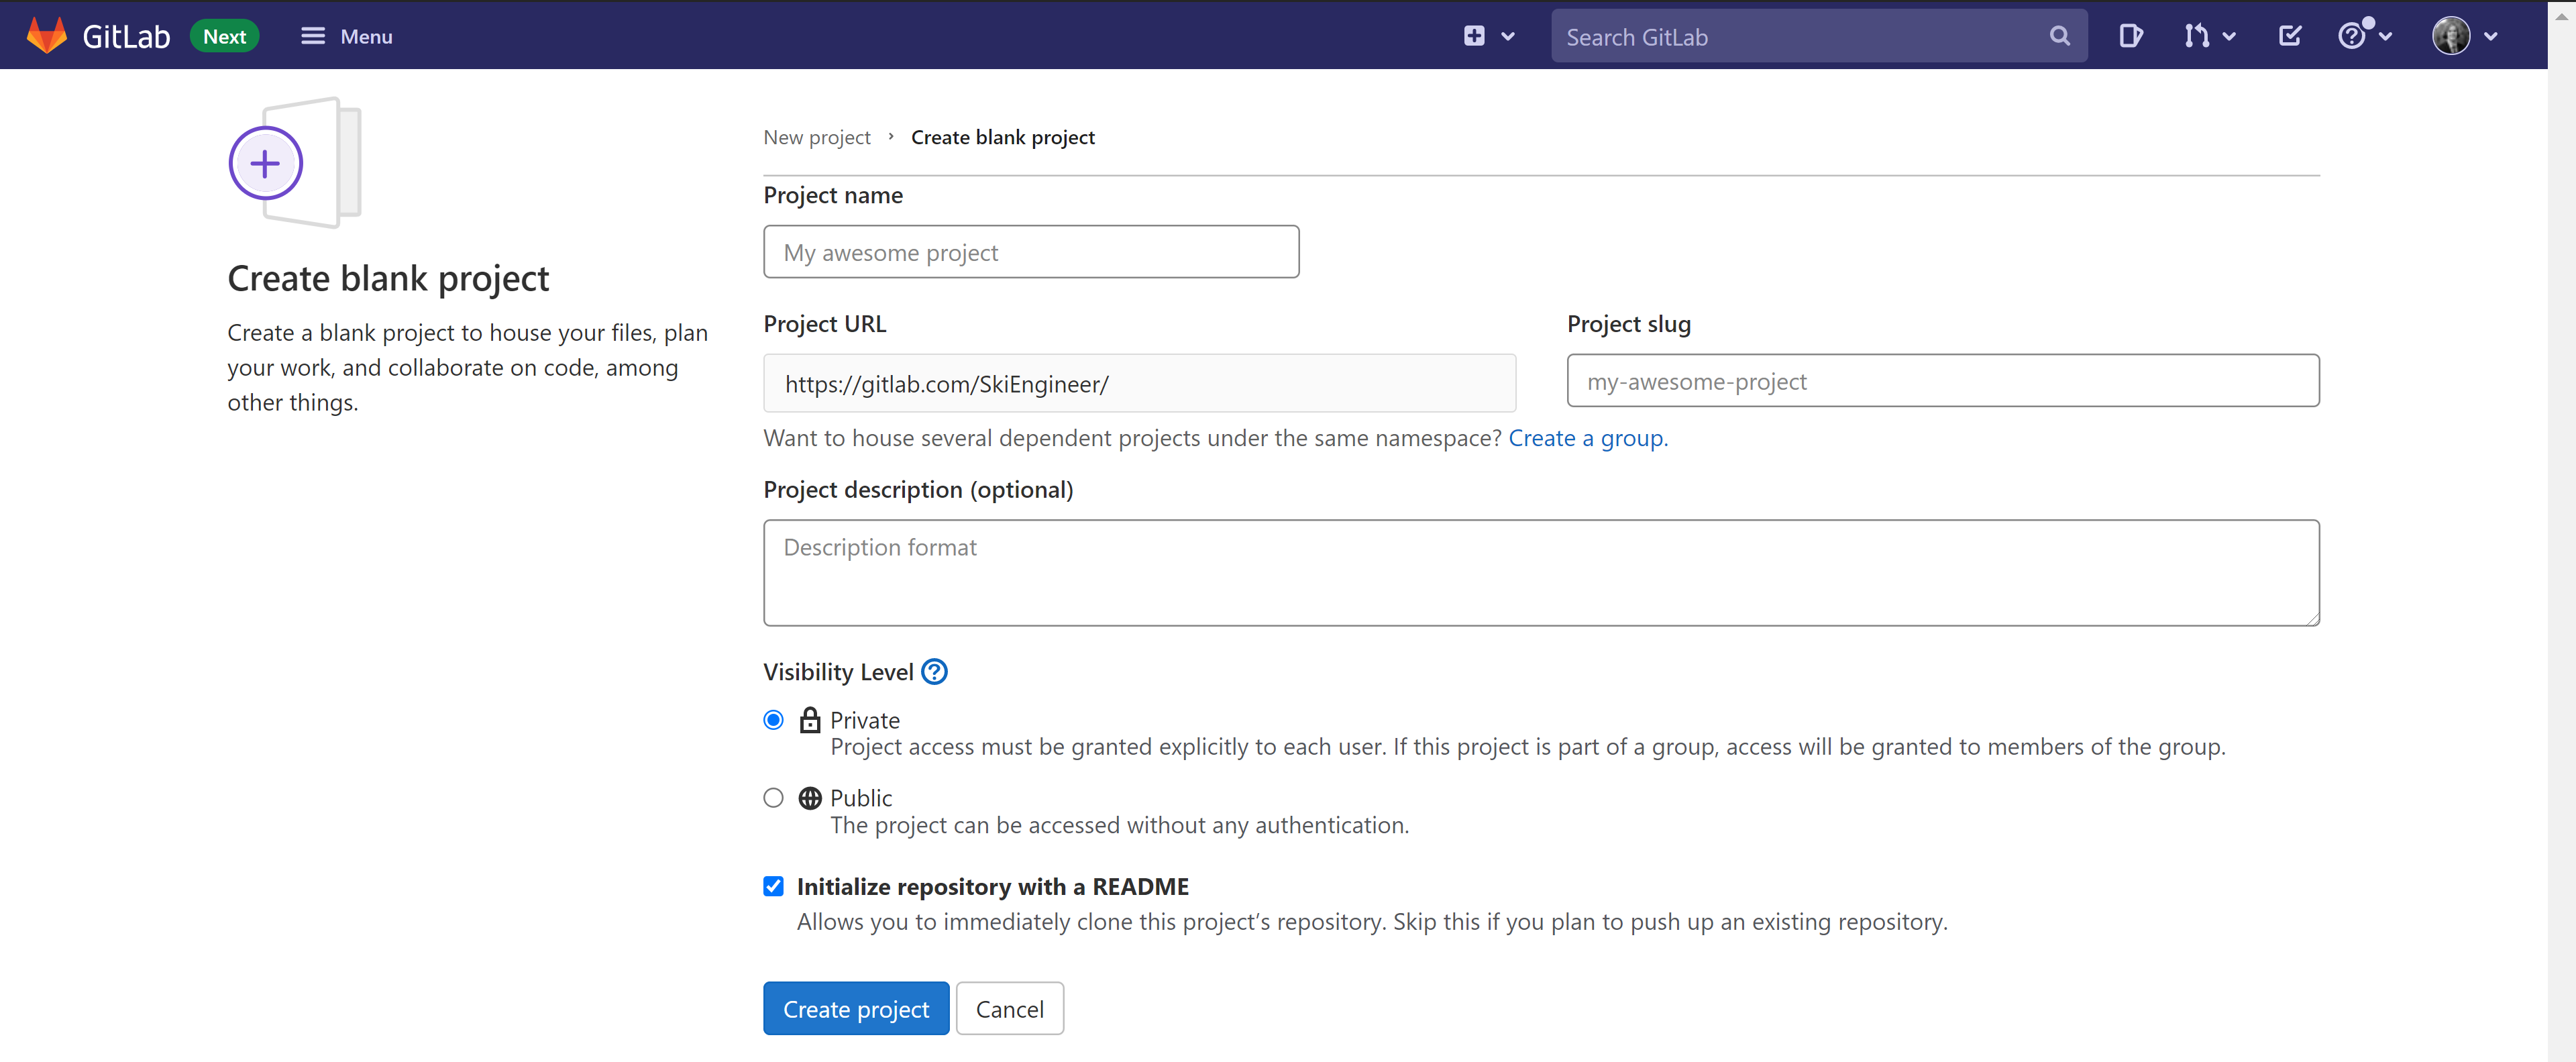
\includegraphics[width=1.0\textwidth]
                {./gitLabProject}
                \caption{Make a new project.}
                \label{fig:gitLabProject}
            \end{figure}
        \item Navigate inside your newly created project
            ``new\_awesome\_project'' directory.  Add the new folder containing
            the copied uofuthesistemplate \texttt{thesis} folder to your own
            repository on \texttt{GitLab}
                {\singlespacing
                \begin{minted}
                    [autogobble,bgcolor=latexcodebg] % 
                    {Bash}
cd ..
cd new_awesome_project
git add thesis
git commit -m "Initial commit of UofU thesis template"
git push
                \end{minted}
                }
    \end{enumerate}

\subsection{Required \texttt{Ubuntu} installations.  Use a \texttt{bash}
    terminal to execute the following commands}
    \begin{enumerate}
        \item Download \texttt{make}
            % \newline
            {\singlespacing
            \begin{minted}
                [autogobble,bgcolor=latexcodebg] % 
                {Bash}
sudo apt-get install build-essential
            \end{minted}
            }
            $\longrightarrow$ The Linux ``\textcolor{blue}{\texttt{make}}''
            command is used to build and maintain groups of programs and files
            from the source code. In Linux, it is one of the most frequently
            used commands by the developers. It assists developers to install
            and compile many utilities from the terminal.
        \item Download \hologo{LaTeX} 
            % \newline
            {\singlespacing
            \begin{minted}
                [autogobble,bgcolor=latexcodebg] % 
                {Bash}
sudo apt install texlive-latex-extra
            \end{minted}
            }
            $\longrightarrow$
            \href{https://linuxconfig.org/how-to-install-latex-on-ubuntu-20-04-focal-fossa-linux}{\hologo{LaTeX}}
            - is a document writing system
        \item Download \hologo{BibTeX} 
            % \newline
            {\singlespacing
            \begin{minted}
                [autogobble,bgcolor=latexcodebg] % 
                {Bash}
sudo apt install texlive-bibtex-extra
            \end{minted}
            }
            $\longrightarrow$
            \href{http://manpages.ubuntu.com/manpages/focal/man1/bibtex.original.1.html}{\hologo{BibTeX}}
            reads the top-level auxiliary (\texttt{.aux})  file auxname  that
            was output  during  the running  of  \texttt{latex}(1)  or
            \texttt{tex}(1)  and  creates a  bibliography  (\texttt{.bbl}) file
            that will be incorporated into the document on subsequent runs of
            \hologo{LaTeX} or \hologo{TeX}.  \\
            
            \hologo{BibTeX} looks up, in bibliographic database (\texttt{.bib})
            files specified by  the  \mintinline{LaTeX}{\bibliography} command,
            the entries  specified by the \mintinline{LaTeX}{\cite} and
            \mintinline{LaTeX}{\nocite} commands in the \hologo{LaTeX} or
            \hologo{TeX} source file.  It formats the information from those
            entries according to instructions in a bibliography  style
            (\texttt{.bst}) file  (specified  by the
            \mintinline{LaTeX}{\bibliographystyle} command, and it outputs the
            results to the \texttt{.bbl} file. \\
            
            The \hologo{LaTeX} manual explains what a \hologo{LaTeX} source
            file  must  contain to  work  with \hologo{BibTeX}.  Appendix  B of
            the \hologo{BibTeX} manual describes the format of the
            \texttt{.bib} files. The `BibTeXing' document describes extensions
            and details of this format, and it gives other useful hints for
            using \hologo{BibTeX}.
        \item Download \texttt{texlive-science} 
            % \newline
            {\singlespacing
            \begin{minted}
                [autogobble,bgcolor=latexcodebg] % 
                {Bash}
sudo apt-get install texlive-science
            \end{minted}
            }
            $\longrightarrow$
            \href{https://packages.ubuntu.com/focal/texlive-science}{\texttt{texlive-science}}
            :  Mathematics, natural sciences, computer science packages
        \item Download \texttt{texlive-fonts-extr} 
            % \newline
            {\singlespacing
            \begin{minted}
                [autogobble,bgcolor=latexcodebg] % 
                {Bash}
sudo apt-get install texlive-fonts-extra
            \end{minted}
            }
            $\longrightarrow$
            \href{https://packages.ubuntu.com/focal/texlive-fonts-extra}{\texttt{texlive-fonts-extra}}
            Additional \hologo{LaTeX} fonts
        \item Download \texttt{biber} 
            % \newline
            {\singlespacing
            \begin{minted}
                [autogobble,bgcolor=latexcodebg] % 
                {Bash}
sudo apt-get install -y biber
            \end{minted}
            }
            $\longrightarrow$
            \href{https://zoomadmin.com/HowToInstall/UbuntuPackage/biber}{\texttt{biber}}
            Much-augmented \hologo{BibTeX} replacement for BibLaTeX users The
            biblatex package by Philipp Lehman is becoming the definitive
            citation management tool for \hologo{LaTeX} users. Biblatex has
            relied on the venerable \hologo{BibTeX} program only for sorting
            and generating a very generic \texttt{.bbl} file without any
            formatting instruction. Everything else is taken care of by
            biblatex, which provides a powerful and flexible macro interface
            for authors of citation styles.  Much-augmented \hologo{BibTeX}
            replacement for BibLaTeX users The biblatex package by Philipp
            Lehman is becoming the definitive citation management tool for
            \hologo{LaTeX} users. Biblatex has relied on the venerable
            \hologo{BibTeX} program only for sorting and generating a very
            generic \texttt{.bbl} file without any formatting instruction.
            Everything else is taken care of by biblatex, which provides a
            powerful and flexible macro interface for authors of citation
            styles.
        \item Download \texttt{Latexmk}
            {\singlespacing
            \begin{minted}
                [autogobble,bgcolor=latexcodebg] % 
                {Bash}
sudo apt-get install -y latexmk
            \end{minted}
            }
            $\longrightarrow$
            \href{http://manpages.ubuntu.com/manpages/bionic/man1/latexmk.1L.html}{\emph{Latexmk}}
            completely  automates the process of compiling a \hologo{LaTeX}
            document.  Essentially, it is like a specialized relative of the
            general  make utility,  but  one  which  determines dependencies
            automatically and has some other very useful features.  In its
            basic mode of operation latexmk is given the name of the primary
            source file  for a  document,  and  it issues  the appropriate
            sequence of commands to generate a .dvi, .ps, .pdf and/or hardcopy
            version of the document.
        \item Download \texttt{Pygments}
            {\singlespacing
            \begin{minted}
                [autogobble,bgcolor=latexcodebg] % 
                {Bash}
sudo apt-get install python3-pygments
            \end{minted}
            }
            $\longrightarrow$ \href{https://pygments.org/}{\emph{Pygments}}
            Pygments is a syntax highlighting engine written in Python. That
            means, it will take source code (or other markup) in a supported
            language and output a processed version (in different formats)
            containing syntax highlighting markup.
            \begin{itemize}
                \setlength\itemsep{0em}
                \item a wide range of over 500 languages and other text formats
                    is supported
                \item special attention is paid to details that increase
                    highlighting quality
                \item support for new languages and formats are added easily;
                    most languages use a simple regex-based lexing mechanism
                \item a number of output formats is available, among them HTML,
                    RTF, \hologo{LaTeX} and ANSI sequences
                \item it is usable as a command-line tool and as a library
            \end{itemize}
    \end{enumerate}

\subsection{Editing Methods For Your Thesis/Dissertation}
    There are two ways you can edit the text of your document:
    \begin{enumerate}
        \item Use \href{https://notepad-plus-plus.org/}{\texttt{Notepad++}} 
            (\cref{fig:Notepad})
            \begin{figure}[H]
                \centering
                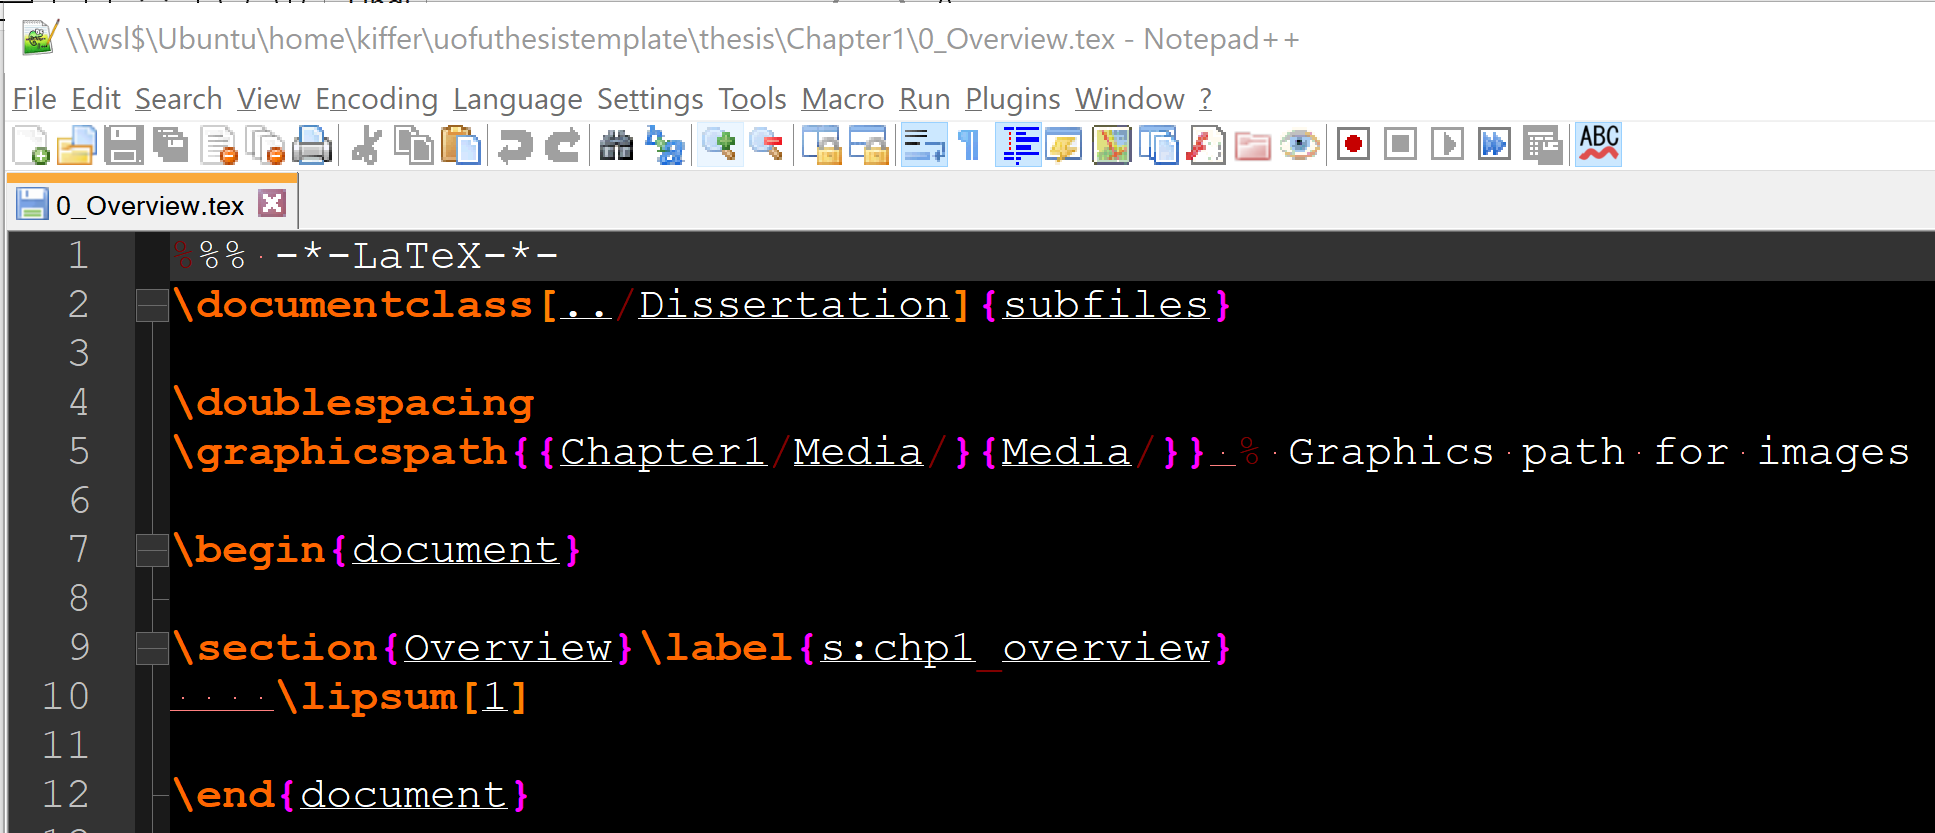
\includegraphics[width=0.9\textwidth]
                {./Notepad}
                \caption{\texttt{Notepad++} editing tool.}
                \label{fig:Notepad}
            \end{figure}
        \item Use
            \href{https://www.tutorialspoint.com/unix/unix-vi-editor.htm}{\texttt{vi}}
            via the command line interface (\emph{Increased efficiency} - Your
            fingers will never leave the keyboard) (\cref{fig:vi_example}).
            \begin{figure}[H]
                \centering
                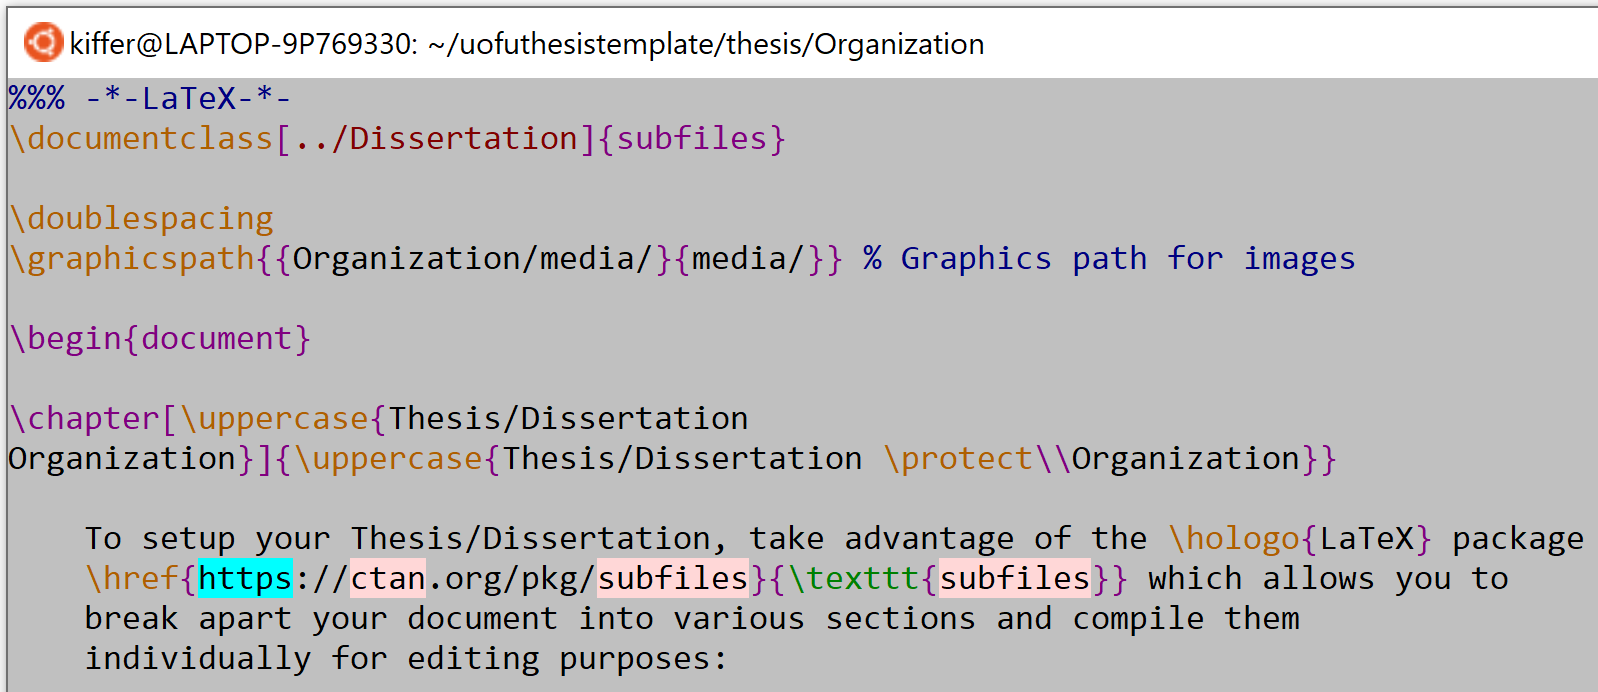
\includegraphics[width=0.9\textwidth]
                {./vi_example}
                \caption{\texttt{vi} editing tool.}
                \label{fig:vi_example}
            \end{figure}
    \end{enumerate}
    
    Add all images/figures to the \texttt{media} folder within each chapter
    
\subsection{How To Make Changes}
    Individual \mintinline{Shell}{makefiles} have been created to execute the
    necessary commands to compile your Thesis/Dissertation.
    
    The basic commands inside of the \mintinline{Bash}{Ubuntu} terminal are:  
    \begin{itemize}
        \setlength\itemsep{0em}
        \item ``\textcolor{blue}{\mintinline{Bash}{make}}'' $\longrightarrow$
            compiles the document.  The associated screen snip in the
            \texttt{Bash} terminal is seen in \cref{fig:LinuxMakeDissertation}
            to compile the Thesis/Dissertation.
        \begin{figure}
            \centering
            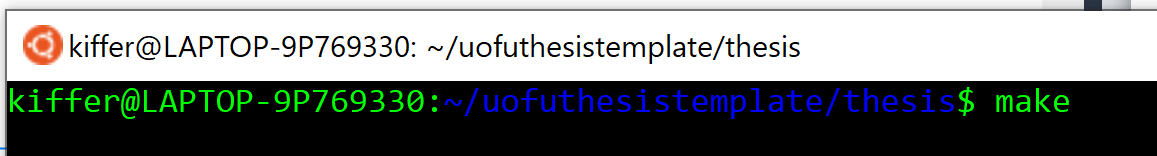
\includegraphics[width=0.9\textwidth]
            {./LinuxMakeDissertation}
            \caption{Screen snip of \texttt{Makefile} command to compile the 
            Thesis/Dissertation.}
            \label{fig:LinuxMakeDissertation}
        \end{figure}
        \item ``\textcolor{blue}{\mintinline{Bash}{make release}}''
            $\longrightarrow$ cleans up the unnecessary files and moves the
            final PDF into the folder titled ``\texttt{Release}''.  To move the
            final PDF into the ``Release'' folder, simply type
            ``\textcolor{blue}{\mintinline{Bash}{make release}}'' and the PDF
            will be moved and the following \hologo{LaTeX} compilation
            documents will be deleted from the folder.  This is seen in
            \cref{fig:LinuxMakeRelease}.
            \begin{figure}
                \centering
                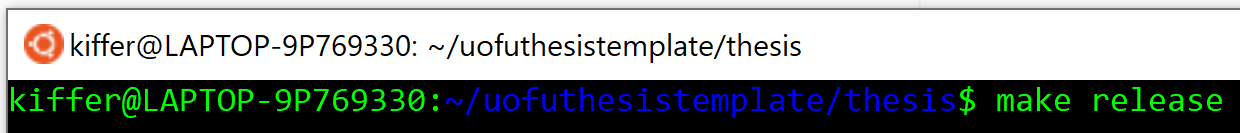
\includegraphics[width=0.9\textwidth]
                {./LinuxMakeRelease}
                \caption{Screen snip of \texttt{Makefile} command to clean up
                the file directory and move the PDF to the ``Release'' folder.}
                \label{fig:LinuxMakeRelease}
            \end{figure}
        \item ``\textcolor{blue}{\mintinline{Bash}{make clean}}''
        \item ``\textcolor{blue}{\mintinline{Bash}{make clear}}''
    \end{itemize}

\subsubsection{Sample \texttt{Makefile}s}
    The following \texttt{Makefile} is used to compile the Thesis/Dissertation:
    
    \codeFromFile{Bash}
        {\subfix{../Makefile}}
        {\ldots \hologo{LaTeX} script used to compile the Thesis/Dissertation.}
        {LaTeXMakefile1}
        {\footnotesize}
        {latexcodebg}
        {default}
    
    The following \texttt{Makefile} is used to compile Chapter 1 of the
    Thesis/Dissertation:
    
    \codeFromFile{Bash}
        {\subfix{../Chapter1/Makefile}}
        {\ldots \hologo{LaTeX} script used to compile Chapter1.}
        {LaTeXMakefile2}
        {\footnotesize}
        {latexcodebg}
        {default}

    The following \texttt{Makefile} is used to compile Chapter 2 of the
    Thesis/Dissertation:
    
    \codeFromFile{Bash}
        {\subfix{../Chapter2/Makefile}}
        {\ldots \hologo{LaTeX} script used to compile Chapter2.}
        {LaTeXMakefile3}
        {\footnotesize}
        {latexcodebg}
        {default}

    The variables in each \texttt{Makefile} are the \hologo{LaTeX} file names
    and you can simply type ``\textcolor{blue}{\mintinline{Bash}{make
    methods}}'' to compile the methods section of a particular chapter.  The
    same is true for ``\textcolor{blue}{\mintinline{Bash}{make abstract}}'',
    ``\textcolor{blue}{\mintinline{Bash}{make results}}'', and
    ``\textcolor{blue}{\mintinline{Bash}{make discussion}}'' which will compile
    the abstract, results, and discussion section, respectively.  This is
    useful for editing sections of the document where you do not necessarily
    need to compile the entire document.  
    
\end{document}
